\chapter{Software Architecture} \label{chap:software_details}

  \section {Use Case View}
    
    The developed application enables the user to create a detailed terrain from a deterministic base surface. To achieve this goal several features, that aid the user in this process, were implemented. This features are specified in Table \ref{table:user_stories} in the form of user stories. Given the nature of this application only one actor, called User, is needed.
    
    
    \begin{table}[h!]
  \centering
  \renewcommand{\arraystretch}{1.5}
  \begin{tabularx}{\linewidth}{|l|l|b|}
	\hline
    \textbf{Code} & \textbf{Name} & \textbf{Description} \\ \hline
    US-001 & Load Base Surface & As a User I want to load a surface from an image so that I can create a detailed version of it. \\ \hline
    US-002 & Export Result & As a User I want to export the result so that I can use it in other applications. \\ \hline
    US-003 & Add Detail & As a User I want to add detail to a previously loaded base surface. \\ \hline
    US-004 & See Result & As a User I want to see my result as I change the parameters so that I can adjust them more easily. \\ \hline
    US-005 & History & As a User I want to be able to consult a list of previously edited terrains so that I can track my work. \\ \hline
    US-006 & History Parameters & As a User I want to have access to the parameters used in previously edited terrains. \\ \hline
    
  \end{tabularx}
  
  \caption{User Stories}
  \label{table:user_stories}
\end{table}
    
    \subsection {User Interface}
    
      The application was developed using Google's material design \cite{Google2016} for the user interface style. The editor is the main page of the application and it is shown in Figure \ref{fig:editor_page}. It contains a menu bar (1) where the user has access to the available functions, a details panel (2), which has the parameter controllers, a list with the previously results (3), a panel where the details of the selected previous result are displayed (4) and a canvas where the preview of the current current terrain is rendered (5).
      
      \begin{figure}[h!]
      	\centering
      	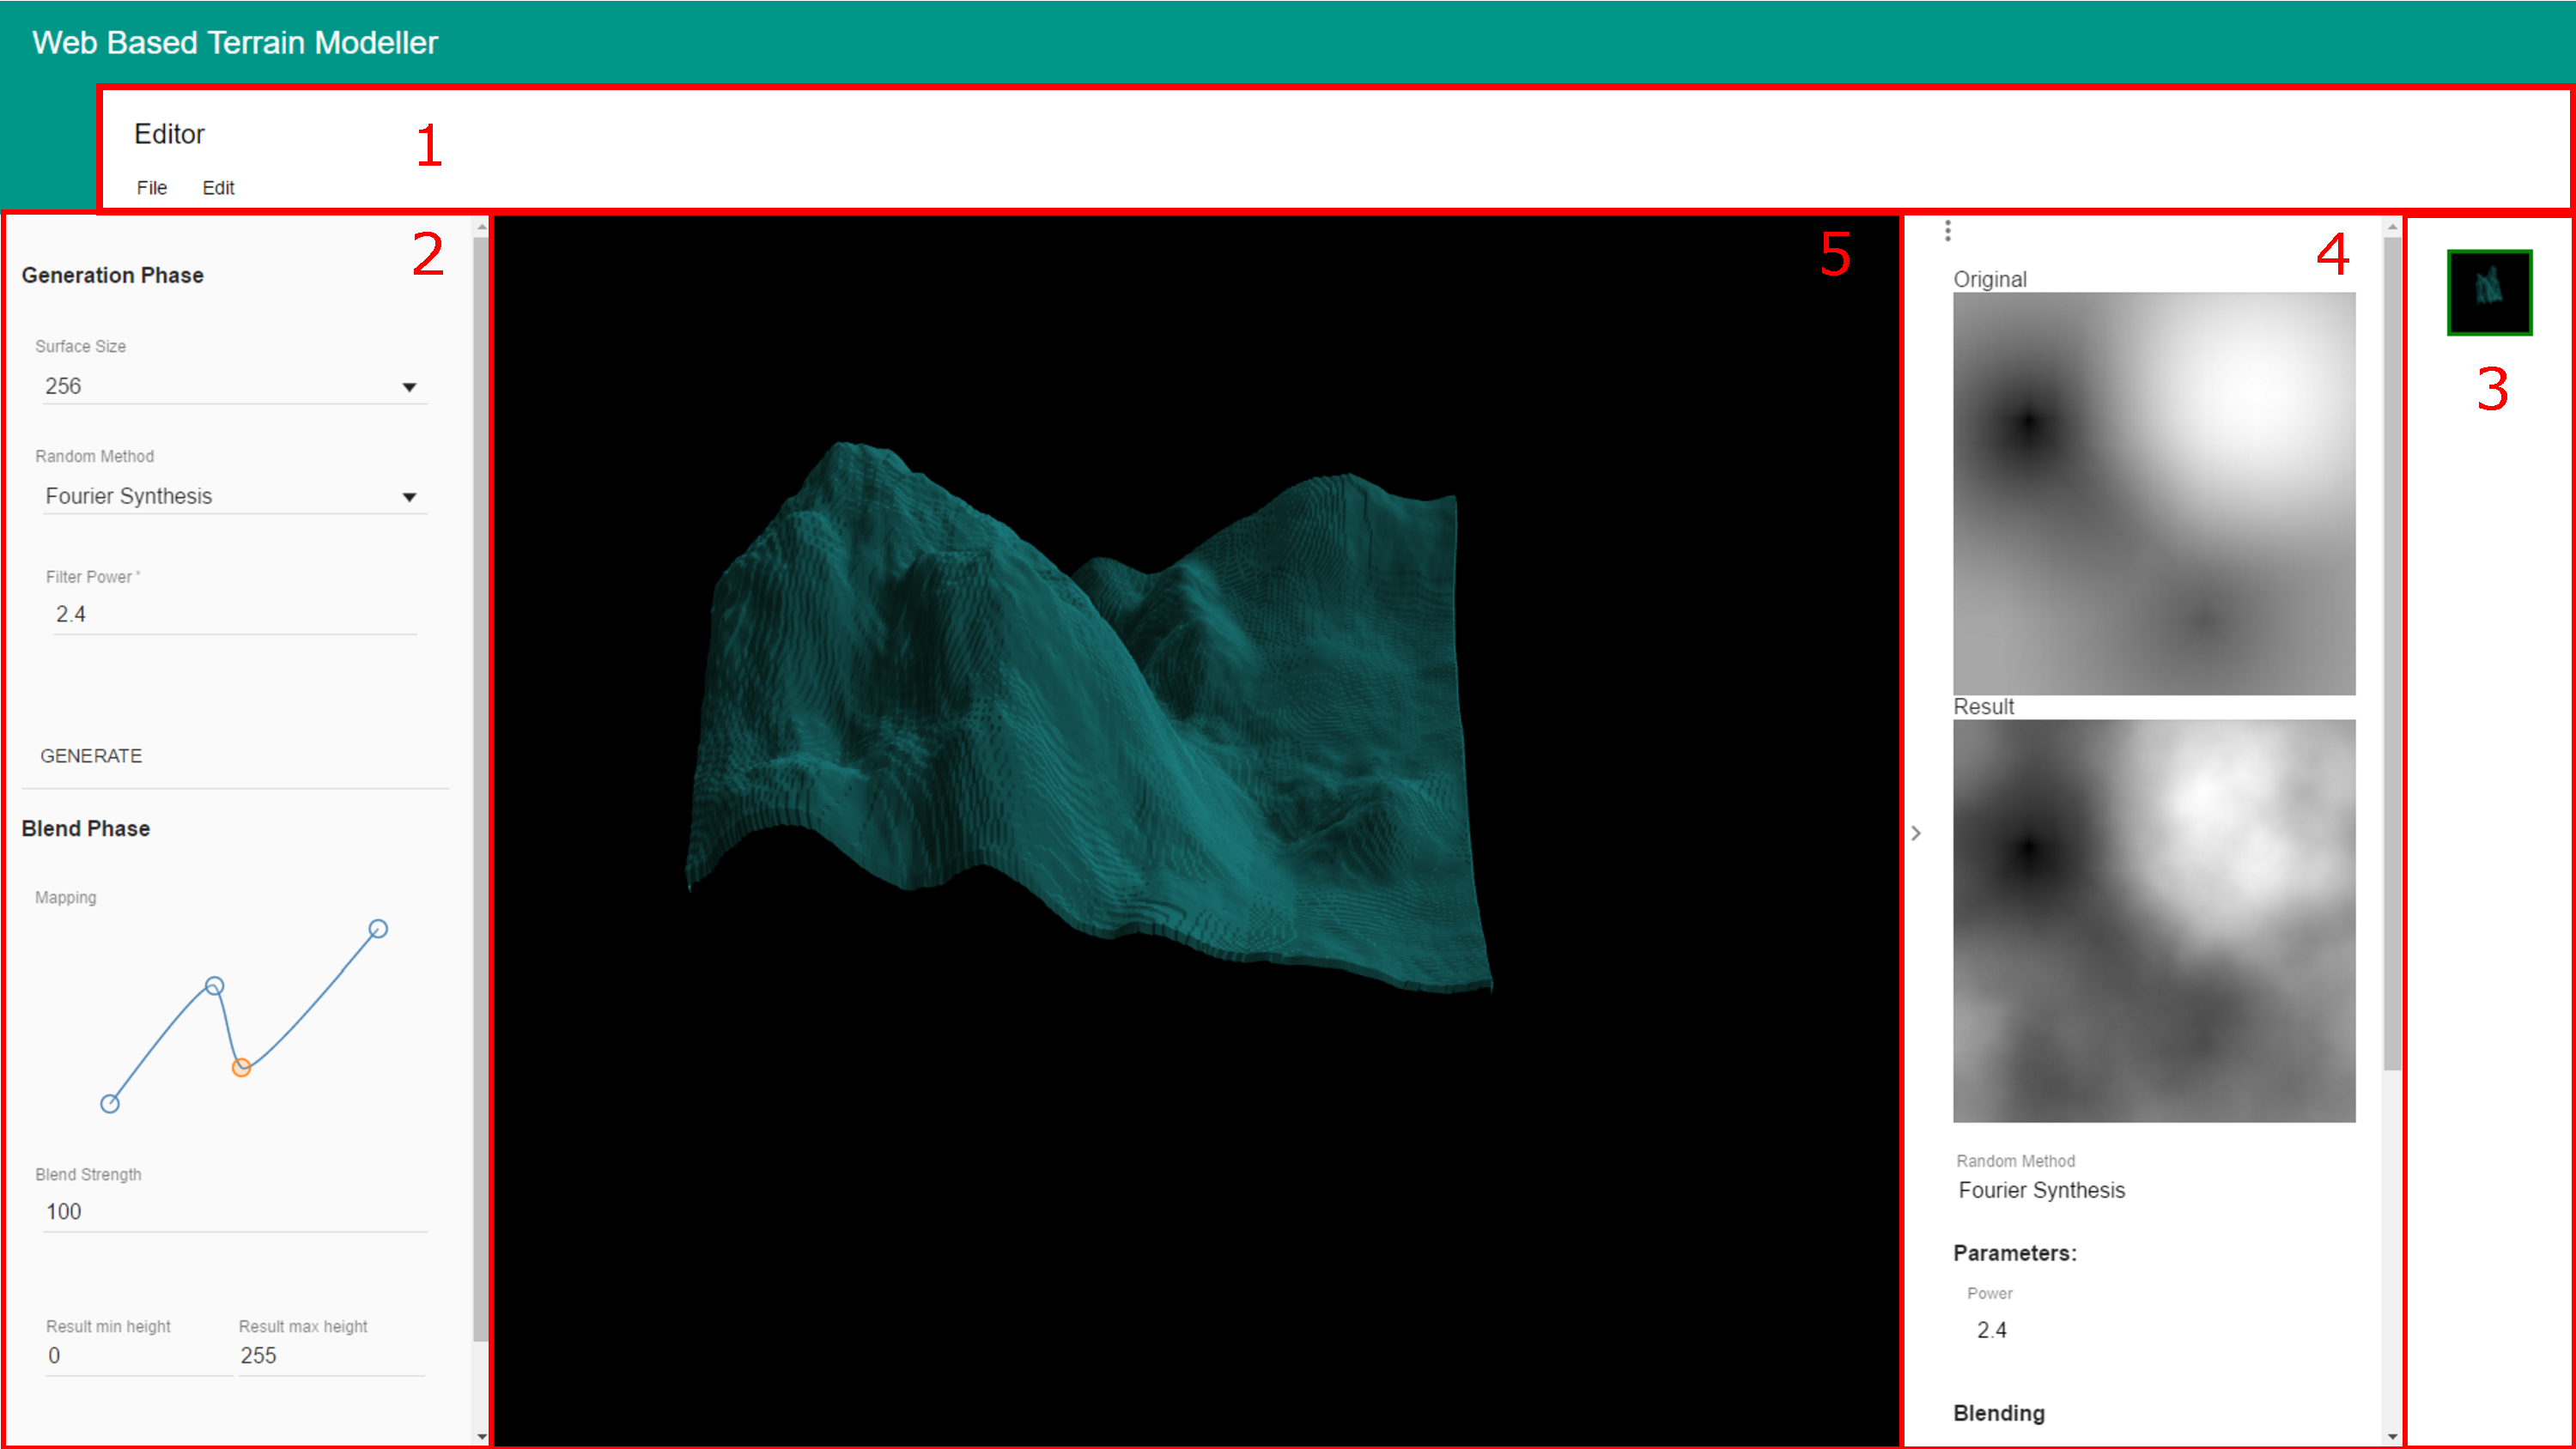
\includegraphics[width=0.95\linewidth]{images/screenshots/editorWithBoxes.pdf}
      	\caption{Editor Page}
      	\label{fig:editor_page}
      \end{figure}
      
      \begin{itemize}
      	\item Explain each panel in detail.
      \end{itemize}
    
    \subsection {Input and Output Formats}
    
      In order to allow the user to load and save his terrains the application implements an import and export feature. The user can either import a Grayscale PNG image, which will be set as the base surface, or import a previously exported Zip file, which will add an entry to the history list and render the result contained in the file. In terms of export formats the user can: obtain: a 4-channel 8-bit per channel PNG containing the height map of the result; a Zip file that can be later imported; and a Grayscale 1-channel 16-bit per channel PNG image of the result height map, which can be import as a landscape in Unreal Engine 4.

  \section {Physical Architecture} %CC Deployment View
    
    The system was developed as a client-side single page web application and thus all the server-side content is static. Given this properties the application works as a static web site and has a simple deployment architecture which consists on a HTTP web server and a web browser, as shown in Figure \ref{fig:deployment_diagram}.
    
    \begin{figure}[h!]
    	\begin{center}
    		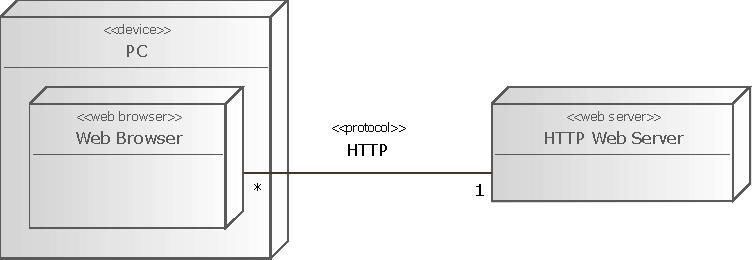
\includegraphics[width=0.9\textwidth]{images/diagrams/deployment.pdf}
    	\end{center}
    	\caption{Deployment Diagram}
    	\label{fig:deployment_diagram}
    \end{figure}
    
  \section {Implementation Architecture} %CC Implementation View
    
    The application is composed by three submodules (Figure \ref{fig:component_diagram}). The \textit{components} submodule is responsible for configuring the page routing and, as such, contains, as submodules, the editor and the benchmarks pages. The \textit{common} module contains services and directives that are generic to the application. The \textit{imgproc} module contains the image processing utilities.
    
    \begin{figure}[H]
      \begin{center}
      	 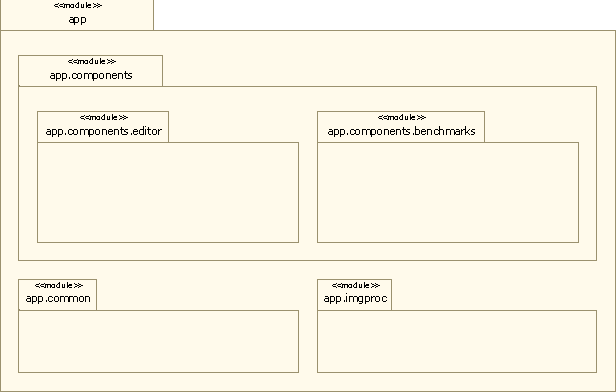
\includegraphics[width=0.9\textwidth]{images/diagrams/component.pdf}
      \end{center}
      \caption{Component Diagram}
      \label{fig:component_diagram}
    \end{figure}


    \subsection {Technologies}    
      
      Given the web-based requirement the application needed to be in Javascript. For convenience the Babel transpiler was used so that the development could be done in ECMAScript 6, which is a newer standard of Javascript. Additionally, to simplify the management of the required dependencies, JSPM and System.js were used, which, integrating with Babel, enable better support for ECMAScript 6 modules. 
      
      To aid the development of the application, Angular.js was used. This framework implements the MVC pattern, which was used to better modularize the source code.
      
      The terrain viewer was implemented using three.js, which is a 3D rendering Javascript library that allows the developer to create 3D Scenes in a straight forward way. 
      
      In order to parallelize some operations, WebGL 2.0 was used. This implementation will be detailed in section \ref{sec:software:process:gpu}
    
  \section {Logical View} %CC Logical View
  
    \begin{itemize}
      \item Angular.JS oriented design
      \item Routes (Directives)
      \item Services
      \item Views
    \end{itemize}
    
  \section {Process View}
    
    \subsection {GPU Computation Framework} \label{sec:software:process:gpu} %CC Process View
    
      \begin{itemize}
      	\item Small introduction to WebGL pipeline
      	\item Generic algorithm execution (Framebuffers \& Textures)
      	\item Matrix Type System
      	\item Implemented Features
      	  \begin{itemize}
      	  	\item FFT \& IFFT
      	  	\item Element-wise Operations
      	  	\item Normalization
      	  	\item Frequency domain filters
      	  	\item Spatial domain filters
      	  \end{itemize}
		\item Radix-2 algorithm for FFT
		\item Reduction based algorithm for finding minimum and maximum
      \end{itemize}
      
    \subsection {Blending Process Pipeline} %CC Process View
    
      \begin{itemize}
      	\item Pseudo-reactive design
      	\item Process diagram
      \end{itemize}